\section{Introduction}

Networks consist of various physical media, topologies, and protocols. 
To manage this complexity effectively, a layered approach is essential.
\begin{figure}[H]
    \centering
    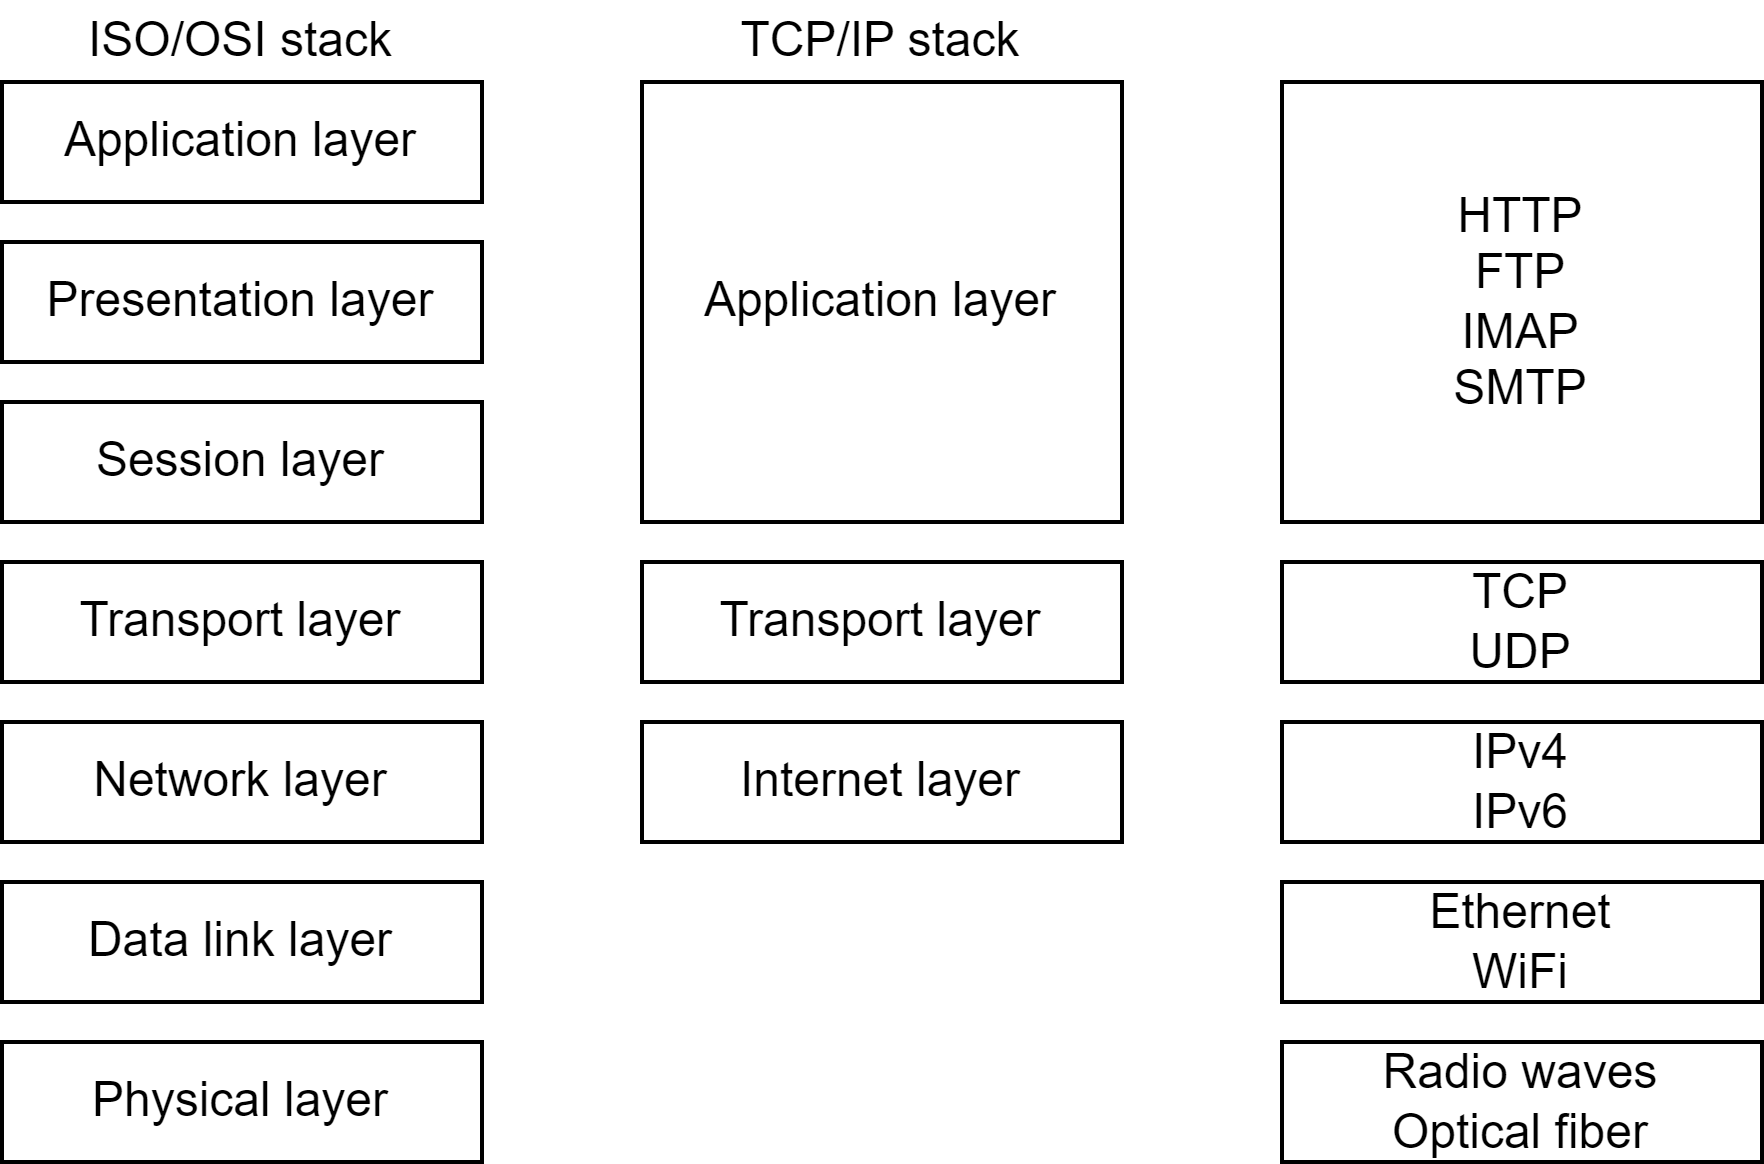
\includegraphics[width=0.75\linewidth]{images/lp.png}
    \caption{Layering and protocols}
\end{figure}

\paragraph*{Addressing}
In network communications, hosts are uniquely identified by their addresses, akin to phone numbers or postal addresses. 
Each network layer employs its own addressing scheme:
\begin{itemize}
    \item \textit{Data link layer}: uses MAC addresses (for Ethernet), a globally unique address embedded in the Network Interface Card (NIC), and the ARP protocol translates an IP address to a MAC address
    \item \textit{Internet layer}: uses IP addresses, identifies a network host globally, and can include private addresses as defined by RFC 1918 for IPv4.
    \item \textit{Transport layer}: uses ports and identifies a specific service on a host.
\end{itemize}

\paragraph*{Transport protocols}
Transport protocols facilitate communication between hosts:
\begin{itemize}
    \item \textit{UDP} (User Datagram Protocol): connection-less, and lightweight wrapper around an IP packet, primarily adding a port number.
    \item \textit{TCP} (Transmission Control Protocol): connection-oriented, and manages state through concepts such as closed, open, and established connections.
        Connections are initiated using a three-way handshake.
\end{itemize}

\subsection{Typical network attacks}
\begin{definition}[\textit{Denial Of Service}]
    A Denial of Service (DoS) attack targets the availability of a service, rendering it inaccessible to legitimate users.
\end{definition}
\begin{definition}[\textit{Sniffing}]
    Sniffing refers to the unauthorized reading of network packets, compromising confidentiality.
\end{definition}
\begin{definition}[\textit{Spoofing}]
    Spoofing involves forging network packets, thereby compromising the integrity and authenticity of communications.
\end{definition}